\chapter{Online Learning Algorithms}
\label{ch:online-learning}\index{online-learning}

\section{Introduction}

\begin{figure}
  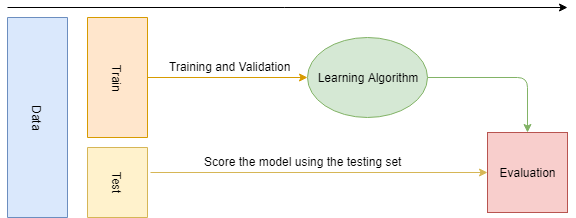
\includegraphics{online_learning/traditional.png}
  \caption{The traditional batch train-test machine learning approach workflow.}
  \label{fig:traditional_ml}
\end{figure}

In the traditional machine learning approach depicted in figure~\ref{fig:traditional_ml}, we usually have some historical data to train an algorithm on for predicting some future events \citep{oza_online_2005}. However, since most data environments are dynamic and will change, the trained model eventually becomes outdated. To tackle this, we usually automate model re-training based on a timeframe (i.e. weekly or daily basis). Although this helps with keeping the model up-to-date, this is still not enough. Even if we consider model re-training on a daily basis, the model would still be at least one day late. To further explain this, let us consider the case study of a recommender engine for an online portal where it shows users items based on their respective preferences. If we consider the situation that one specific item has gone globally viral overnight, our recommender system will fail to display this item to the whole population and instead would show the item to a part of the user-base.
Moreover, after re-training the following day, the recommender engine would start pushing this item to the entire population, even though this item might no longer be relevant. Thus, our traditional algorithm has failed twice merely because it was slow to react to the dynamic change in item relevance. Furthermore, as \citet{pagels_what_2018} argued, no matter how good a specific model is, it would always be an imperfect representation of the problem. Furthermore, to have the best prediction for today, we cannot rely on a model with knowledge about yesterday only. Enter online learning algorithms, a family of techniques that are modelled to consume as much data available (one sample at a time), as fast as possible, while continuously learning and adapting different learning parameters. The next section we will discuss the following questions: why use online learning? Also, most importantly, when?

\section{Synthesis}

\begin{figure}
  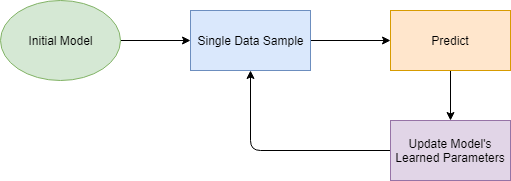
\includegraphics{online_learning/online.png}
  \caption{Basic workflow architecture of online learning.}
  \label{fig:online_ml}
\end{figure}

\subsection{Why use Online Learning?}

While being highly adaptable to dynamic underlying data structures since they make no statistical assumptions on the distribution of the data \citep{hoi_libol:_2014}, online learning techniques are also highly data efficient. Since online learning algorithms are only updated using the most recent data samples in the stream (as illustrated in figure~\ref{fig:online_ml}), such data samples are no longer stored or needed once the algorithm has passed over them, maintaining a much smaller data storage \citep{oza_online_2005}. Such algorithms are also very fast since only a single pass on a smaller data set is made, in contrast to the standard approach where the optimisation function needs multiple iterations over the entire dataset. Thus, as argued by \citet{hoi_online_2018}, online learning algorithms scale much better than the traditional approach.

\subsection{When to use Online Learning?}

Although online learning techniques are widely adopted in all areas of machine learning tasks \citep{hoi_online_2018}, below we will discuss some situations were online learning would drastically improve our model, based on the properties as discussed above.

\begin{enumerate}
\item \textbf{Large Data Volume -} \index{online-learning!data volume} As aforementioned, in offline machine learning, we load an entire dataset in memory, process it and then train a specific model, and then deploy the model into production. However, as more and more data is being generated, especially with the bright spotlight on Big Data, this methodology is proving to be more and more tedious. Some data sets are too large to fit into memory, even with distributed computing measures in place. Thus, online learning can drastically help in this scenario due to its small data storage property, especially when considered as online distributed computing and out-of-core computation \citep{zhang_projection-free_2017}.

\item \textbf{Time-Series Data -} \index{online-learning!time-series} Most of our real-life data sets are represented and based as a function of time (i.e. measuring the same parameters over time). As highlighted in the previously mentioned case study, this task fits perfectly with online learning. To be able to make predictions of the present, we must have a model that is also knowledgeable about the present, as close to real-time as possible \citep{hoi_online_2018, Lane:1998:AOL:3000292.3000339}.

\item \textbf{Data Distribution Morphism -} \index{online-learning!data morphism} Another important feature of online learning is its fast adaptability, making this methodology useful for tasks with high data velocity, susceptible of concept drift (the evolution of underlying patterns and relationships in the data, i.e. evolution of user behaviour with time) \citep{hoi_online_2018, Lane:1998:AOL:3000292.3000339}.
\end{enumerate}

\subsection{Challenges of Online Learning}

Even though most online learning algorithms are designed for fast execution speeds and are thus adapted from less complex algorithms, implementation challenges are also present. One of the most significant problems in online learning as highlighted by \citet{gepperth_incremental_2016} is catastrophic interference, where the model abruptly forgets knowledge learnt for previous data. Most online learning algorithms allow the user to set a forgetting rate, which depicts the speed at which the learning algorithm forgets older data. Moreover, the correct calibration of this rate is essential and challenging to perfect since a high value would result in catastrophic interference, while a lower value would result in the algorithm not adapting to the incoming samples in the stream. In addition to this, good initialisations are critical in this approach to steer away from slow convergence.

\section{Conclusion}

In this chapter, we introduced and discussed the sub-field of online learning algorithms concerning machine learning. Online learning is a highly useful tool that allows us to take machine learning to a whole other level by solving problems that otherwise would seem to be out of our technical ability. With the exponential importance for Big Data analytics, online learning arms us with the capabilities to process high-velocity data while also being fast to adapt to frequent changes in the data.